\documentclass[12pt]{article}
\usepackage[utf8]{inputenc}
\usepackage{float}
\usepackage[margin=1in]{geometry}
\usepackage[utf8]{inputenc}
\usepackage{graphicx}
\usepackage{subcaption}
\usepackage{ amsmath }
\usepackage{mathtools,etoolbox}
\usepackage{ amssymb }
\usepackage[utf8]{inputenc}
\usepackage[T1]{fontenc}
\usepackage{bbold}

\title{3-21-19 Summary (Temperatures Fixed)}
\author{Haina Wang, Charles Maher}

\begin{document}

\maketitle

\section{Virial Expansions}

Our results from low density simulations agree well with the $S(0)$ derived from the pressure virial expansions, and the slightly larger k behavior derived from the $g_2$ virial expansions. Following is a table comparing $S(0)$ from several vapor phase simulations and the virial expansion up to the second virial coefficient, as well as plots comparing the $g_2$ virial expansions to both the simulated $g_2$ and $S(k)$. In both cases, the virial expansions predict that the $S(0)$ will be greater than unity. 
\begin{table}[H]
\centering
\caption{Comparison of $S(0)$ simulation to the virial expansion up to the first order.}
\begin{tabular}{|l|l|l|}
\hline
Parameters (T, $\rho$) & S(0): Simulation & S(0): First Order Virial Expansion \\ \hline
0.741, 0.0163        & 1.49508          & 1.4356                             \\ \hline
0.777, 0.0235        & 1.68572          & 1.64019                            \\ \hline
0.803, 0.030         & 1.89925          & 1.85031                            \\ \hline
0.857, 0.053         & 2.60935          & 3.30699                            \\ \hline
0.893, 0.09          & 5.47402          & -12.8853                           \\ \hline
\end{tabular}
\end{table}

\begin{figure}[H]
		\centering
		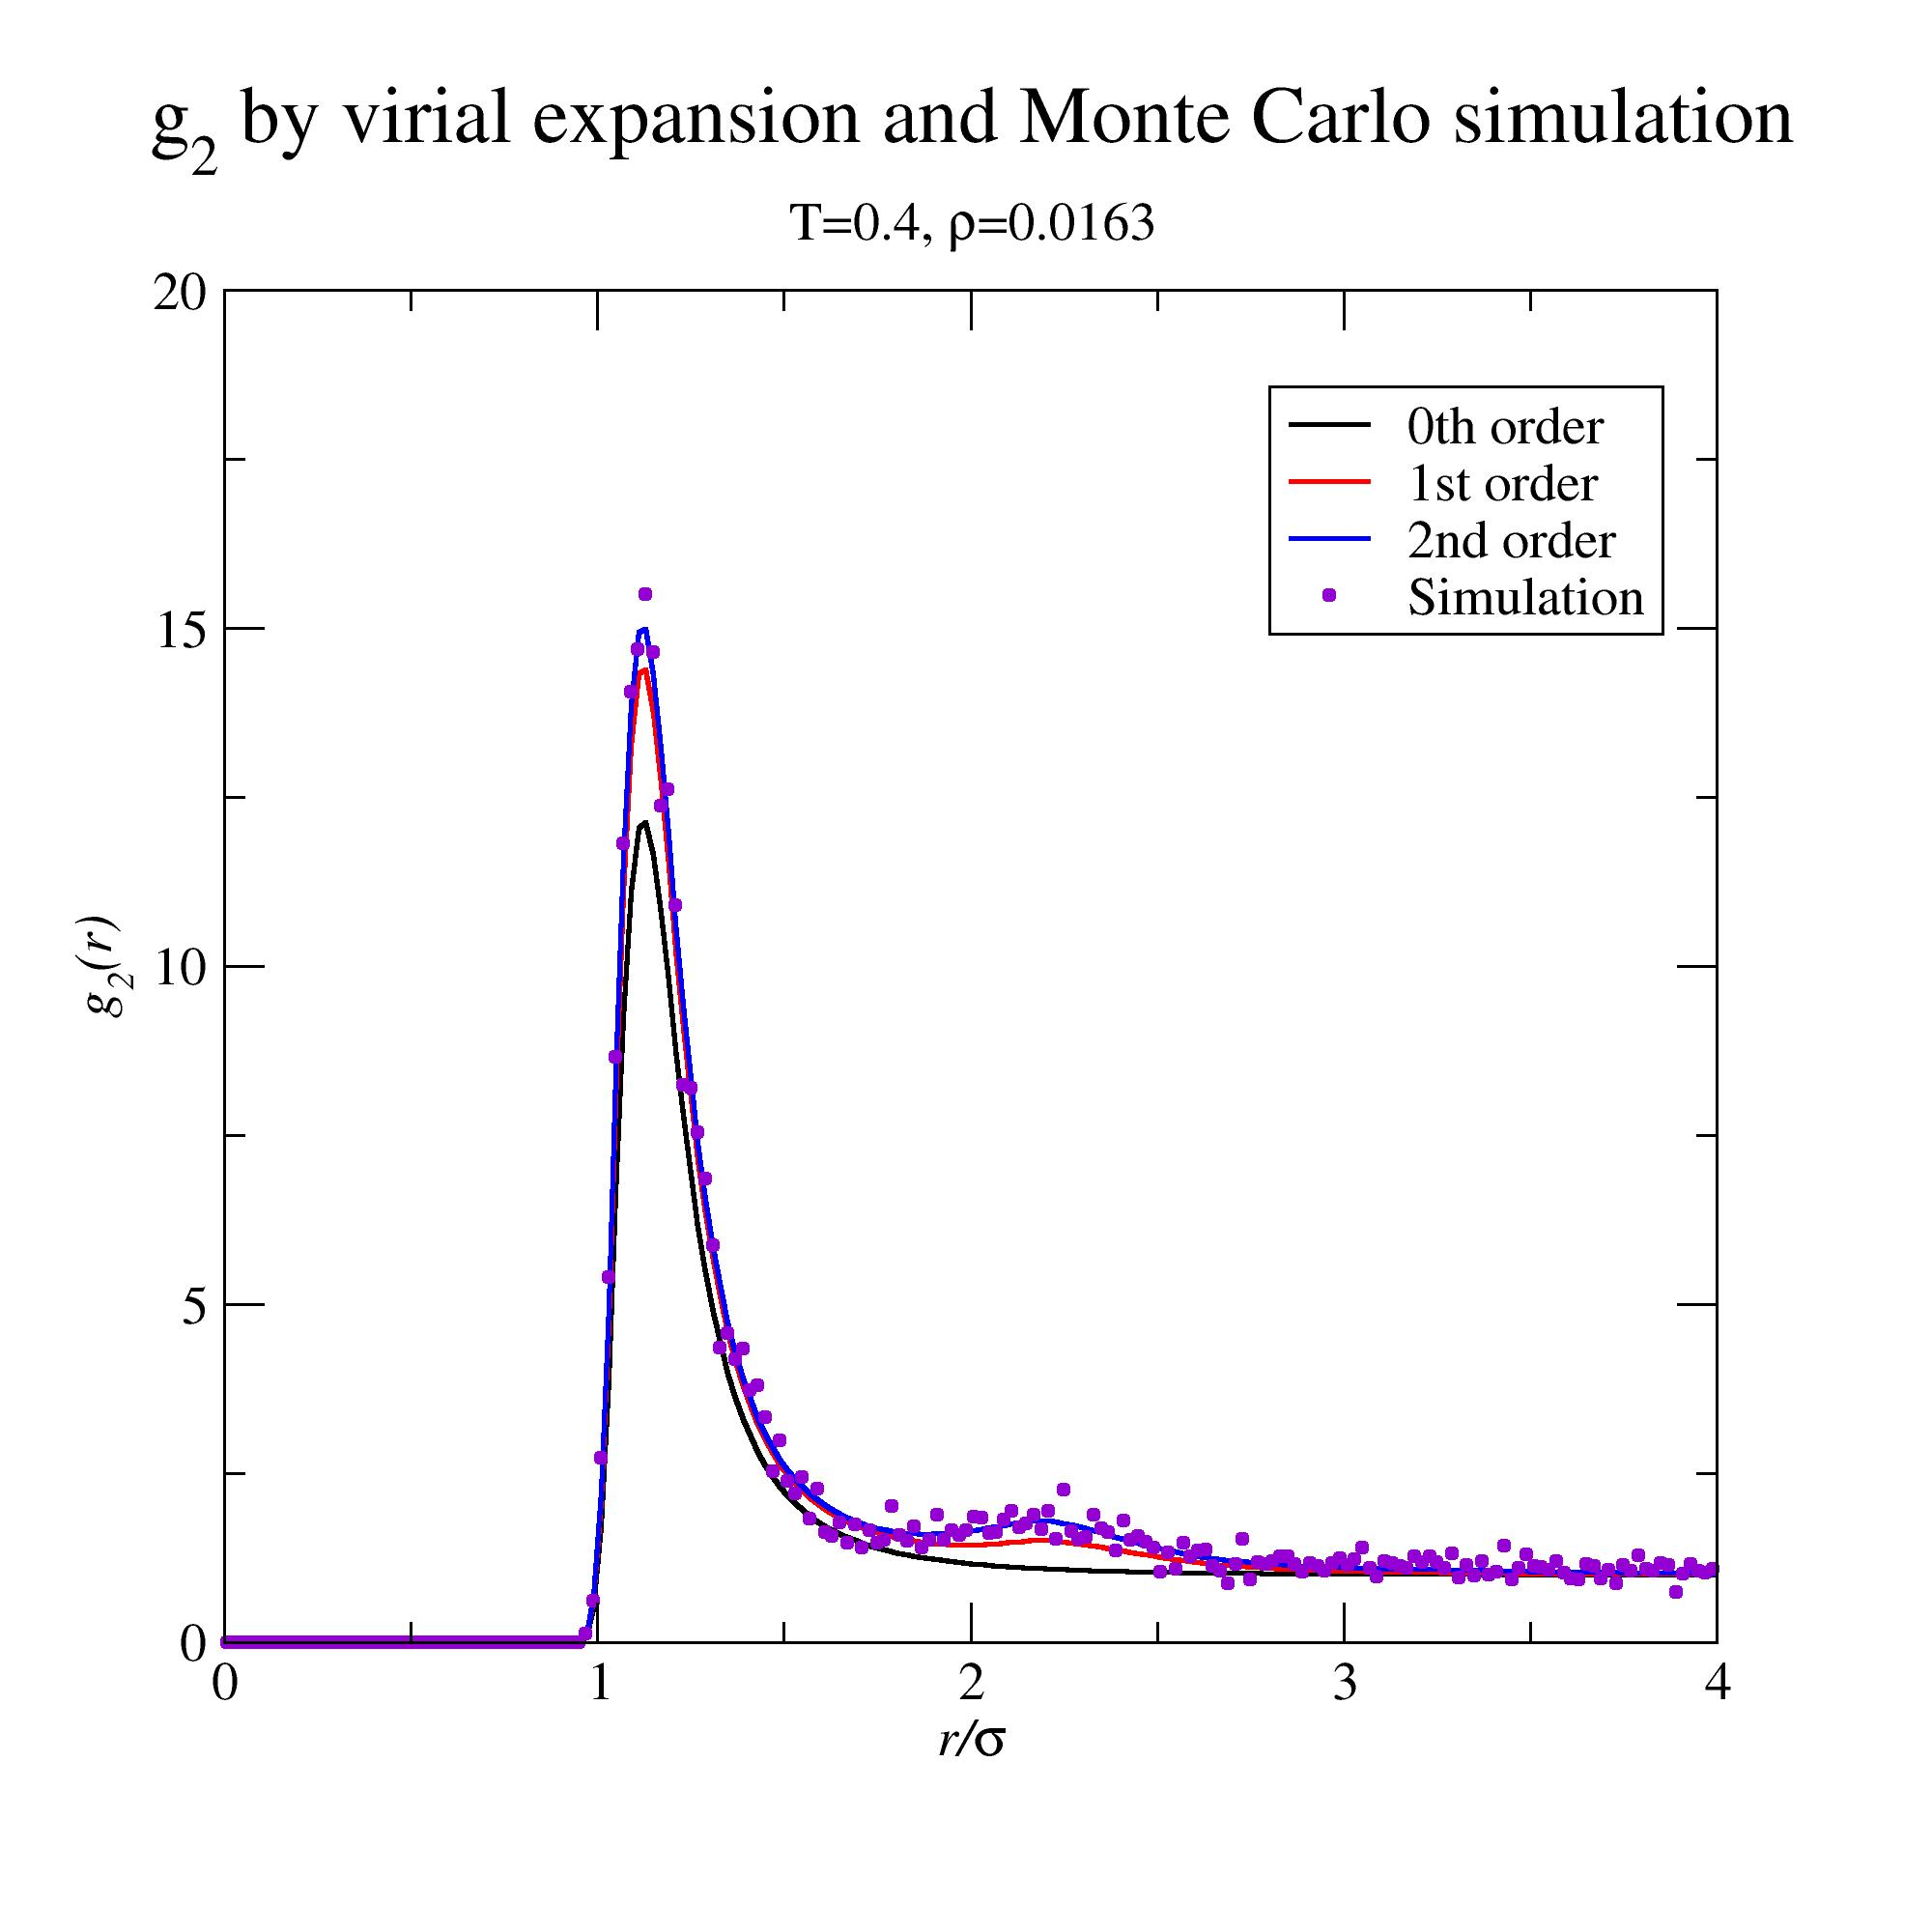
\includegraphics[width=0.7\linewidth]{g2rho0x0163t0x40}
		\label{fig:g2rho0x0163t0x40}
\end{figure}

\begin{figure}[H]
		\centering
		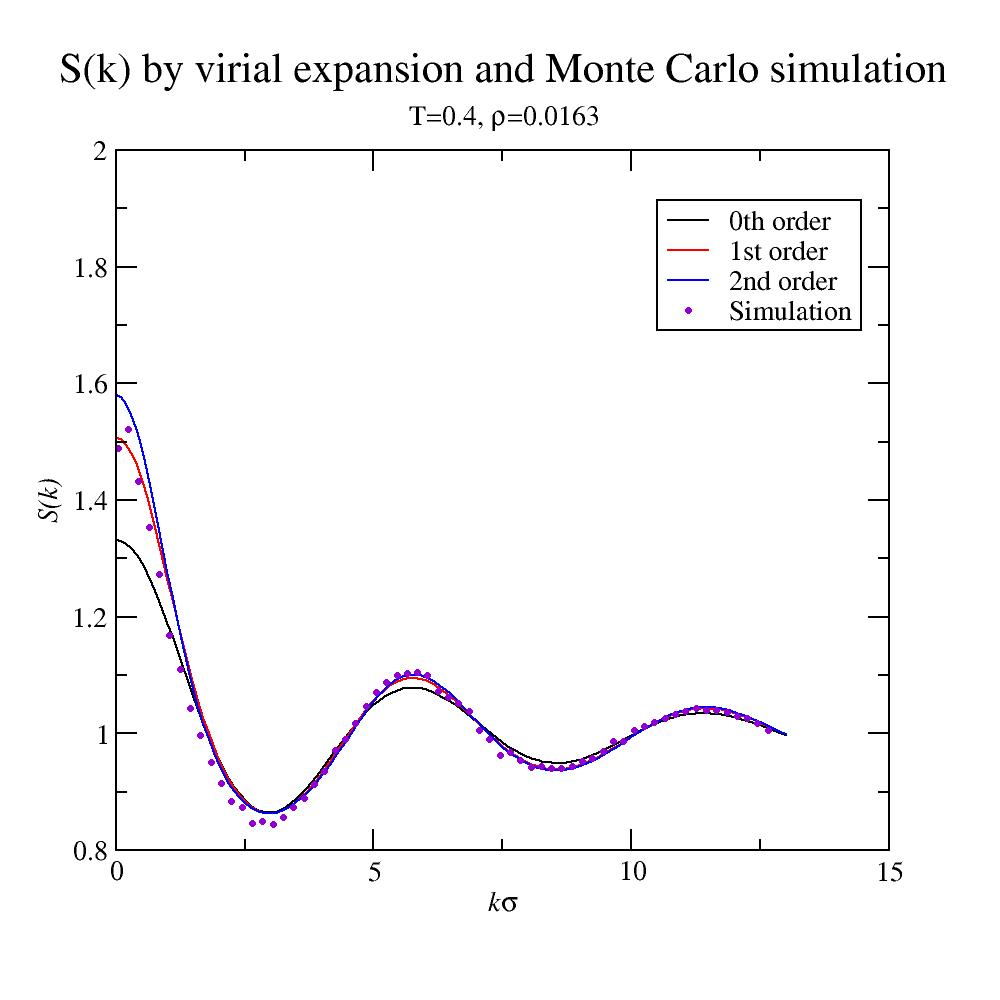
\includegraphics[width=0.7\linewidth]{Skrho0x0163t0x40}
		\label{fig:Skrho0x0163t0x40}
\end{figure}
\noindent
Using these results we can corroborate our simulation results for low density in the vapor phase, but have no strict theoretical confirmation for higher density vapor simulations, or the liquid phase simulations. This "low density" cut-off will depend on the temperature of the system, but for the temperatures we tend to use for the simulations the cutoff density is around $\rho$ = 0.05.

The virial expansion's convergence to the simulated $g_2$ is much slower according to Glandt's studies at a higher density, with $\rho=0.32, T=1.25$.

\subsection{Uncertainty of $T_c$}
According to Glandt (1978), virial expansions underestimate the critical density. 

Subject to truncation and shifting criteria used, the critical temperature vary in different papers, ranging from 0.459 (Smit 1990) to 0.625 (Tsien 1974). We tentatively accept $T_c=0.56$ in Henderson (1977), using full LJ potentials (truncation radius $\geq6.5\sigma$). 

\section{The liquid side}
For all simulations of liquids that we have performed, the first peak of $S(k)$ at nonzero $k$ is higher than $S(0)$, but $S(0)$ can rise above 1 for less dense liquids. 

For the same density, $S(0)$ increases as $T$ decreases. 

For simulations with $N=400$, the temperatures and densities at which $S(0)=1$ seem to have a linear relation regardless of the states of matter, as shown in the following graph. 

\begin{figure}[H]
		\centering
		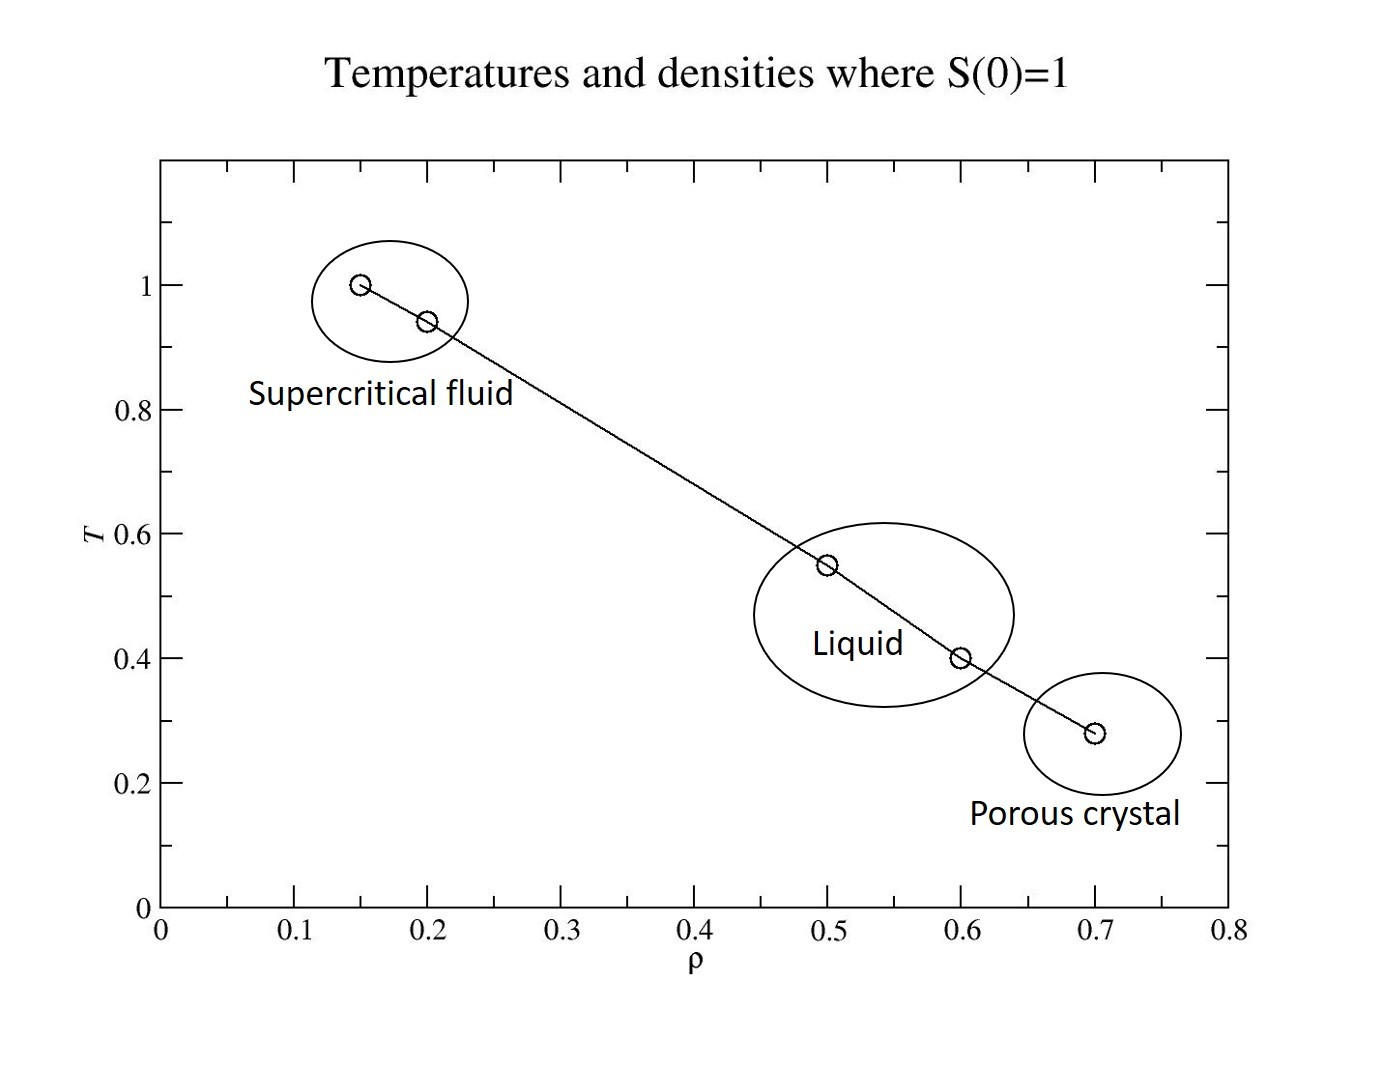
\includegraphics[width=0.7\linewidth]{fallBelow1.jpg}
		\label{fig:fallBelow1}
\end{figure}

The reason of this behavior (whether physical or computational) as well as whether it persists for other system sizes is still to be answered.

\section{S(k) with Fixed Temperatures}
\begin{figure}[H]
    \centering
    \includegraphics[width=6in]{032019LJVaporAlongDome.eps}
    \caption*{$S(k)$ for several points along the liquid-vapor coexistence line on the vapor side. $S(0)$ increases quickly as the critical point is approached.}
\end{figure}

\begin{figure}[H]
    \centering
    \includegraphics[width=6in]{032019LJLiquidAlongDome.eps}
    \caption*{$S(k)$ for several points along the liquid-vapor coexistence line on the liquid side. $S(0)$ seems to also increase as the critical point is approached, but to a much smaller degree than in the liquid. The amount of noise in this compared to the liquid is likely a result of the simulation box being smaller, allowing for fewer $k$ sampling points in the same window. This can be remedied by simulating more particles, and I will begin running these simulations.}
\end{figure}
\end{document}
